% =============================================================
%   MINOR PROJECT REPORT — B.Tech (Phase-II, 6th Semester)
%   Dr. B. R. Ambedkar National Institute of Technology Jalandhar
%   Department of Instrumentation and Control Engineering
% =============================================================
\documentclass[12pt,a4paper,oneside]{report}

% ─── Packages ────────────────────────────────────────────────
\usepackage[margin=1in,top=1.2in,bottom=1.2in]{geometry}
\usepackage{times}          % Times New Roman style
\usepackage{graphicx}
\usepackage{amsmath, amssymb}
\usepackage{booktabs}
\usepackage{longtable}
\usepackage{array}
\usepackage{multirow}
\usepackage{xcolor}
\usepackage{hyperref}
\usepackage{setspace}
\usepackage{titlesec}
\usepackage{enumitem}
\usepackage{fancyhdr}
\usepackage{caption}
\usepackage{subcaption}
\usepackage{listings}
\usepackage{algorithm}
\usepackage{algpseudocode}
\usepackage{tocloft}
\usepackage{float}
\usepackage{cite}
\usepackage{parskip}
\usepackage{microtype}
\usepackage{mdframed}
\usepackage{tabularx}
\usepackage{pifont}

% ─── Hyperref Setup ──────────────────────────────────────────
\hypersetup{
    colorlinks=true,
    linkcolor=black,
    citecolor=black,
    urlcolor=blue,
    pdftitle={Intelligent Pesticide Sprinkling System},
    pdfauthor={Bhavesh Singh, Chahat Kesharwani, Sadgi Saraswat, Vanshika Soni},
}

% ─── Line Spacing ────────────────────────────────────────────
\onehalfspacing

% ─── Header / Footer ─────────────────────────────────────────
\pagestyle{fancy}
\fancyhf{}
\rhead{\small Intelligent Pesticide Sprinkling System}
\lhead{\small Minor Project Report}
\cfoot{\thepage}
\renewcommand{\headrulewidth}{0.4pt}
\renewcommand{\footrulewidth}{0.4pt}

% ─── Chapter / Section Formatting ────────────────────────────
\titleformat{\chapter}[display]
  {\normalfont\Large\bfseries\centering}
  {\chaptertitlename\ \thechapter}{12pt}{\Large}
\titlespacing*{\chapter}{0pt}{10pt}{20pt}

\titleformat{\section}{\normalfont\large\bfseries}{\thesection}{1em}{}
\titleformat{\subsection}{\normalfont\normalsize\bfseries}{\thesubsection}{1em}{}
\titleformat{\subsubsection}{\normalfont\normalsize\itshape}{\thesubsubsection}{1em}{}

% ─── Code Listing Style ──────────────────────────────────────
\lstset{
  basicstyle=\ttfamily\footnotesize,
  keywordstyle=\color{blue}\bfseries,
  commentstyle=\color{gray},
  stringstyle=\color{orange!80!black},
  frame=single,
  breaklines=true,
  numbers=left,
  numberstyle=\tiny\color{gray},
  captionpos=b
}

% ─── Custom Commands ─────────────────────────────────────────
\newcommand{\HRule}{\rule{\linewidth}{0.5mm}}
\newcommand{\keyword}[1]{\textbf{#1}}

% ─────────────────────────────────────────────────────────────
\begin{document}

% ─── Plain style for front matter ────────────────────────────
\pagestyle{empty}

% =============================================================
%  TITLE PAGE
% =============================================================
\begin{titlepage}
\begin{center}

\vspace*{0.5cm}
{\large \textbf{MINOR PROJECT REPORT (PHASE -- II)}}\\[0.3cm]
{\normalsize B.Tech 6\textsuperscript{th} Semester}\\[0.6cm]
\HRule\\[0.3cm]
{\LARGE \textbf{Intelligent Pesticide Sprinkling System\\
Determined by the Infection Level of Plants}}\\[0.3cm]
\HRule\\[0.8cm]

\textit{Submitted by}\\[0.3cm]
\begin{tabular}{ll}
\textbf{Bhavesh Singh}      & (23106030) \\
\textbf{Chahat Kesharwani}  & (23106032) \\
\textbf{Sadgi Saraswat}     & (23106078) \\
\textbf{Vanshika Soni}      & (23106099) \\
\end{tabular}\\[0.8cm]

\textit{Under the Supervision of}\\[0.3cm]
{\large \textbf{Dr. Karan Veer}}\\
\textit{Assistant Professor}\\
\textit{Department of Instrumentation and Control Engineering}\\[1.0cm]

% Institute Logo placeholder

\includegraphics[width=0.2\linewidth]{logo_250.png}\\[0.6cm]


{\large \textbf{Department of Instrumentation and Control Engineering}}\\
{\large \textbf{Dr. B. R. Ambedkar National Institute of Technology Jalandhar}}\\
Jalandhar, Punjab -- 144008\\[0.3cm]
{\normalsize \textit{Academic Year 2025--2026}}

\end{center}
\end{titlepage}

% ─── Roman page numbering begins after title page ─────────────
\pagenumbering{roman}
\setcounter{page}{1}
\pagestyle{plain}

% =============================================================
%  CERTIFICATE PAGE
% =============================================================
\newpage
\phantomsection
\addcontentsline{toc}{chapter}{CERTIFICATE}
\begin{center}
{\Large \textbf{CERTIFICATE}}
\end{center}
\vspace{1cm}

\noindent This is to certify that the minor project entitled \textbf{``Intelligent Pesticide Sprinkling System Determined by the Infection Level of Plants''} has been carried out by:

\vspace{0.5cm}
\begin{center}
\begin{tabular}{ll}
Bhavesh Singh      & (23106030) \\
Chahat Kesharwani  & (23106032) \\
Sadgi Saraswat     & (23106078) \\
Vanshika Soni      & (23106099) \\
\end{tabular}
\end{center}
\vspace{0.5cm}

\noindent under my supervision and guidance in partial fulfilment of the requirements for the degree of Bachelor of Technology in Instrumentation and Control Engineering at Dr. B. R. Ambedkar National Institute of Technology Jalandhar during the academic year 2025--2026.

\noindent To the best of my knowledge and belief, the work is original, has not been submitted to any other institution, and has not been published earlier.

\vspace{2.5cm}
\noindent
\begin{tabular}{p{0.45\textwidth}p{0.45\textwidth}}
\textbf{Project Supervisor} & \textbf{Project Coordinator (PRC)} \\[1.5cm]
\rule{5cm}{0.4pt} & \rule{5cm}{0.4pt} \\
Dr. Karan Veer & \\
Assistant Professor & \\
Dept. of ICE, NIT Jalandhar & \\
\end{tabular}


% =============================================================
%  ACKNOWLEDGEMENT
% =============================================================
\newpage
\phantomsection
\addcontentsline{toc}{chapter}{ACKNOWLEDGEMENT}
\begin{center}
{\Large \textbf{ACKNOWLEDGEMENT}}
\end{center}
\vspace{0.8cm}

\noindent We express our heartfelt gratitude and sincere thanks to \textbf{Dr. Karan Veer}, Assistant Professor, Department of Instrumentation and Control Engineering, NIT Jalandhar, for his invaluable guidance, constant encouragement, constructive feedback, and unwavering support throughout the course of this minor project. His technical expertise and insightful suggestions were instrumental in shaping the direction and quality of this work.

\noindent We extend our sincere thanks to the \textbf{Head of the Department of Instrumentation and Control Engineering} and all faculty members for providing the necessary resources, laboratory facilities, and academic environment required for the completion of this project.

\noindent We also acknowledge the support of \textbf{NIT Jalandhar} for providing access to computational resources, high-speed internet, and the campus garden environment used for prototype testing.

\noindent Finally, we are deeply grateful to our \textbf{families and peers} for their moral support and encouragement throughout this academic endeavour.

\vspace{2cm}
\noindent
\begin{tabular}{ll}
Bhavesh Singh      & (23106030) \\
Chahat Kesharwani  & (23106032) \\
Sadgi Saraswat     & (23106078) \\
Vanshika Soni      & (23106099) \\
\end{tabular}

% =============================================================
%  TABLE OF CONTENTS
% =============================================================
\newpage
\pagestyle{fancy}
\tableofcontents

% =============================================================
%  MAIN BODY BEGINS
% =============================================================
\newpage
\pagenumbering{arabic}
\setcounter{page}{1}

% =============================================================
\chapter{INTRODUCTION}
% =============================================================

\section{Background and Motivation}

Agriculture forms the cornerstone of India's economy, providing employment to about
58% of rural workers and making significant contributions towards the GDP of the country. To
provide food security for the growing population, not only high yielding crops are required but
also efficient utilization of resources in agriculture. One of the major issues faced by farmers is
that of disease management of plants. Failure in the prevention of plant diseases can lead to
the loss of crops by 20%-80% according to the types of plants used and intensity of infection [5].
Pesticides and chemical solutions have long been the main weapons in battling plant disease and
pests. The traditional method of pesticides' use is quite wasteful in itself, using a spray system
that applies the solution to the entire field irrespective of the plant's health conditions. This not
only leads to wasting huge amounts of pesticides since much of the applied pesticides do not
even make contact with their target organisms [1], but also results in environmental degradation
due to damage to non-target organisms and soil pollution.

The tomato (\textit{Solanum lycopersicum}) is one of the most economically relevant vegetable crops produced around the world. It is very vulnerable to various types of diseases such as Early Blight (\textit{Alternaria solani}), Late Blight (\textit{Phytophthora infestans}), Septoria Leaf Spot, and Tomato Yellow Leaf Curl Virus (TYLCV). If these diseases are not properly detected and controlled at an early stage, they can result in heavy financial losses due to their quick proliferation across the entire plot of the crop.

Thanks to recent developments in artificial intelligence, deep learning technology, and embedded systems, precision farming can now explore novel avenues for its advancement. Various machine learning algorithms, especially CNNs, have proven to possess impressive capabilities in disease identification using image data of leaves. In combination with IoT-based automated actuation mechanisms, they can become the core of closed-loop spraying devices that will use pesticides only when required.
% =============================================================
\chapter{LITERATURE REVIEW}
% =============================================================

\section{Overview}

This chapter presents previous literature and technologies associated with plant diseases detection, precision agriculture, and automatic pesticide applications.

\section{Waste of Pesticides and Environmental Impacts}

The waste of pesticides had been widely analyzed by Lyseng [1]. They identified that a significant percentage of the chemicals used in spraying does not reach the desired plants because of wind drift, chemical runoff, and evaporation, which led to significant financial loss and severe pollution of the environment for farmers. Their analysis indicated that there is a need for developing a smart system for helping the farmers in applying pesticides to the desired plants only.
Environmental impacts of using pesticides without control were studied by Healy et al. [3] through their project called PestMan. They found out that applying environmentally friendly techniques in spraying results in a significant reduction in the chemicals' runoffs from the fields. However, it is worth noting that they did not include any technology associated with plant disease detection and spraying.

\section{Machine Learning-Based Plant Disease Detection}

The deep learning-based ensemble framework comprising ResNet50 and MobileNetV2 by Kumar
et al. [5] for tomato leaf disease classification provides excellent results in terms of classification accuracy. Unfortunately, this model can be employed only for offline disease identification but does not
include severity analysis and interaction with the pesticide application system.
The study of Ibrahim et al. [4] is devoted to the design of AI-IoT-based smart agriculture that aims
to provide an automated disease detection and treatment system using convolutional neural net-
works trained on cloud servers and connected to IoT-based sensors providing environmental
information. In spite of their success in automated disease detection, this study lacks a proportional
pesticide administration scheme since the quantity of pesticide used depends on the extent of
disease propagation.

\section{Robotic and Automated Spraying Systems}

According to Pansare et al. [2], an intelligent agricultural robot capable of identifying diseases in plants and activating the process of applying pesticides was suggested. While this approach has shown how disease identification could be effectively combined with pesticide application processes with the aid of robotics, several limitations should also be noted here. First of all, the implementation of such an approach required high costs; secondly, it entailed certain complications, and, thirdly, the amount of applied pesticides was not proportional to the level of spreading of disease among plants. As a result, the amount of pesticides used for each plant regardless of infection rate remained the same. Another approach by Ahmed [6] was also based on the development of a pest management system in the field of smart agriculture. In spite of its effectiveness in terms of integrating environmental sensors and pest identification, no methods for image recognition were used in this case. The ensemble-based deep learning method using ResNet50 and MobileNetV2 for detecting diseases on tomato leaves introduced by Kumar et al. [5] seems rather promising in regard to the accuracy of the task. Nevertheless, this approach allows determining diseases in an offline environment and does not take into consideration the issue of the spread of the disease and administering of pesticides.
As mentioned in the work of Ibrahim et al. [4], a smart agriculture technology incorporating AI-IoT systems and designed for automating the processes of disease detection and pesticides administration in order to treat these plants was offered in this study. Even though the researchers managed to develop an automatic disease detection and treatment system using CNN models and IoT-based sensors, the proportionality of applying pesticides is not taken into account.

\section{Automated Pesticide Spraying Systems}

As Pansare et al. [2] noted, a smart robot for precision farming capable of detecting plant diseases and automatically spraying the necessary pesticides was created. Although this study proves that it is feasible to incorporate both technologies in robotic solutions, some downsides have been identified in terms of this project, such as a relatively high price of the system, a complicated technology, and lack of ability to determine the amount of pesticides depending on the area of infection. Moreover, all plants affected by diseases received an equivalent amount of pesticides despite the level of infections. In comparison, Ahmed [6] designed pest management for precision farming with the use of smart IoT-based sensors.


% =============================================================
\chapter{PROBLEM STATEMENT AND RESEARCH GAP}
% =============================================================

\section{Detailed Problem Statement}

\subsection{What is the Problem?}

Traditional pesticide usage within agricultural systems is inherently inefficient since a blanket spray is applied to the whole area without taking into account the state of health of each particular plant. Consequently, this leads to:

\begin{enumerate}[label=,itemindent=\parindent,leftmargin=3.5em]
\item \textbf{An excessive application of pesticides to healthy and slightly diseased plants.}
\item \textbf{Insufficient use of pesticides for severely diseased plants.}
\item \textbf{Delaying in the treatment process} caused by dependence on manual examination and consequently the spread of diseases. 
\item \textbf{A great financial load on farmers} because of unnecessary purchase of chemicals.
\item \textbf{Polluting the environment} through pesticide overflow and its absorption by the soil. 
\end{enumerate}


\subsection{Why is it Important?}

\begin{itemize}[leftmargin=2em]
    \item India loses approximately 15--25\% of its annual agricultural produce to plant diseases.
    \item WHO estimates that 3 million cases of pesticide poisoning occur annually worldwide, with 220,000 deaths.
    \item Excessive pesticide use contributes to biodiversity loss, including bee colony collapse, threatening food chain stability.
\end{itemize}

\subsection{Who is Affected?}

\begin{itemize}[leftmargin=2em]
    \item \textbf{Small and marginal farmers} who spend disproportionately on pesticides relative to income.
    \item \textbf{Consumers} exposed to pesticide residues on food.
    \item \textbf{Ecosystems} impacted by chemical contamination of soil and water.
    \item \textbf{Agricultural workers} at risk of chronic pesticide exposure.
\end{itemize}

\subsection{Proposed Solution}

The proposed solution is a \textbf{Pesticide Sprinkling System using an Intelligent Model} which consists of:

\begin{enumerate}[leftmargin=2em]
    \item Image capture of tomato leaves using a camera.
    \item Image preprocessing and classification using a fine-tuned EfficientNetV2-M model based on three categories: \textbf{healthy}, \textbf{moderate infection}, and \textbf{severe infection}.
    \item Transmission of the image classification results through Wi-Fi to an ESP32 microcontroller.
    \item Activation of a pump-valve nozzle based on the severity level for a calibrated time period.
    \item Recording of all activity on a real-time web interface.
\end{enumerate}

\section{Research Gap}

A key research gap addressed by this project is:

\begin{mdframed}[linewidth=1pt, linecolor=black!70, backgroundcolor=gray!8]
\textit{There are no affordable and modular systems currently that can perform both (1) real-time machine learning-based classification of infection severity on tomato leaves, and (2) proportional actuation based on severity for the application of pesticides using a closed-loop control strategy.}
\end{mdframed}

Specifically, the gap includes the following points:

\begin{itemize}[leftmargin=2em]
    \item \textbf{Actuation gap:} Current devices either detect presence of a disease (binary classification) without varying the amount of pesticide delivered.
    \item \textbf{Integration gap:} Machine learning modules and actuation devices are seldomly combined to form one system.
    \item \textbf{Cost gap:} Solutions offered in scientific literature are prohibitively expensive and cannot be implemented by smaller institutions.
    \item \textbf{Scalability gap:} Most solutions have little room for scalability to work with other plants and fields.
\end{itemize}

% =============================================================
\chapter{SCOPE AND OBJECTIVES}
% =============================================================

\section{Scope of the Project}

\subsection{What is Included}

\begin{itemize}[leftmargin=2em]
    \item Implementation of image-based machine learning classification for detecting the level of infection in tomatoes' leaves.
    \item Implementation of a spraying actuator using an ESP32 microcontroller.
    \item Establishment of a wireless Wi-Fi communication link between the inference engine and the actuator.
    \item Implementation of a real-time web dashboard for monitoring purposes.
    \item Conducting experiments on a controlled garden site on campus.
    \item Application of tomato leaf diseases' dataset acquired from Kaggle and Plant Village online platforms.
    \item Employing a combination of water and a safe dye as a substitute for pesticides.
\end{itemize}

\subsection{What is Excluded}

\begin{itemize}[leftmargin=2em]
    \item Full-scale field deployment on commercial agricultural land.
    \item Disease detection for crops other than tomatoes (reserved for future work).
    \item Development of a fully autonomous mobile navigation system (manual cart positioning is used).
    \item Economic impact analysis or full life-cycle cost assessment.
    \item GPS-based geo-tagging of infected plants.
\end{itemize}

\subsection{Constraints}

\begin{tabular}{p{3cm}p{10cm}}
\textbf{Time:} & 6-month project duration (6\textsuperscript{th} semester). \\
\textbf{Budget:} & Limited to publicly available datasets and low-cost hardware (ESP32, 12V pump, nozzles). \\
\textbf{Environment:} & Controlled campus garden and laboratory conditions. \\
\textbf{Dataset:} & Limited to tomato leaf images; model accuracy depends on dataset diversity. \\
\textbf{Connectivity:} & Requires stable Wi-Fi network for ESP32-laptop communication. \\
\end{tabular}

\section{Objectives of the Project}

\begin{enumerate}[leftmargin=2em, label=\textbf{O\arabic*.}]
    \item To train and develop an ML model using the EfficientNetV2-M framework via transfer learning for classification of the tomato plant disease condition into three classes: \textbf{Healthy}, \textbf{Moderate Infection} (30–60\% leaf area coverage), and \textbf{Severe Infection} ($>$60\% leaf area coverage) with the desired classification accuracy being $\geq$ 90\%.

    \item To design an automated and real-time system for pesticide application via ESP32 microcontroller-based regulation of pump working duration in accordance with the ML model severity predictions.

    \item To interface the ML prediction module with the physical hardware controller via HTTP request over Wi-Fi connection protocol with a system response time not exceeding 5 seconds from image capture to the start of spraying process.

    \item To save at least \textbf{40\%} of pesticide usage as compared to uniform spraying techniques through the designed prototype during testing on a set of tomato test plants of different infection degrees.

    \item To provide a live web dashboard logging health conditions, spraying operations performed on each plant, timestamps, and overall pesticide usage.

    \item To build a modular, scalable, and economically viable prototype of the pesticide sprayer, keeping the total hardware cost under \textbf{Rs. 5,000}.
\end{enumerate}

% =============================================================
\chapter{METHODOLOGY}
% =============================================================

\section{System Overview and Architecture}

The proposed Intelligent Pesticide Sprinkling System follows a modular, five-stage pipeline architecture as illustrated in Figure \ref{fig:block_diagram}. The system operates as a closed-loop control framework where visual inputs drive mechanical outputs through an intelligent decision layer.


\begin{figure}[H]
\centering
    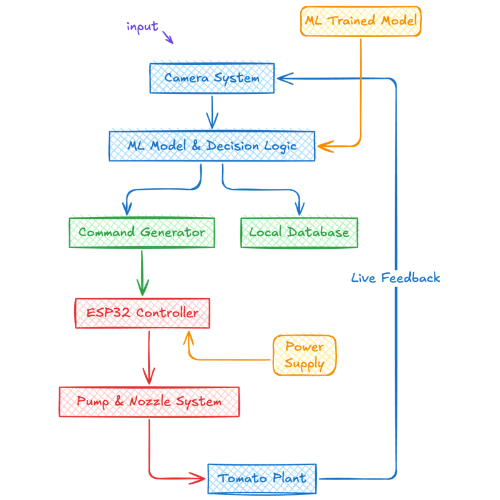
\includegraphics[width=0.87\linewidth]{blockdia.png}
\caption{High-Level System Block Diagram of the Intelligent Pesticide Sprinkling System}
\label{fig:block_diagram}
\end{figure}

The five modules are:

\begin{enumerate}[leftmargin=2em]
    \item \textbf{Module 1:} Image Capture \& Preprocessing
    \item \textbf{Module 2:} ML-Based Infection Severity Detection
    \item \textbf{Module 3:} Decision Logic \& Communication
    \item \textbf{Module 4:} Spraying Actuation System
    \item \textbf{Module 5:} Monitoring \& Logging Dashboard
\end{enumerate}



\section{Complete System Workflow: Step-by-Step}

\begin{algorithm}[H]
\caption{Intelligent Pesticide Sprinkling System Workflow}
\label{alg:main_workflow}
\begin{algorithmic}[1]
\State \textbf{Initialize:} Load EfficientNetV2-M model, start Flask server, connect ESP32 to Wi-Fi
\For{each plant in the garden row}
    \State Position mobile cart adjacent to plant $i$
    \State Capture leaf image $\mathbf{I}_i$ using USB camera
    \State Preprocess $\mathbf{I}_i$: resize, normalize, denoise $\rightarrow \hat{\mathbf{I}}_i$
    \State Pass $\hat{\mathbf{I}}_i$ through EfficientNetV2-M $\rightarrow$ softmax probability vector $\mathbf{p}_i$
    \State $\hat{y}_i \leftarrow \arg\max(\mathbf{p}_i)$ \Comment{Predicted severity class}
    \State Map $\hat{y}_i$ to spray duration $t_s$ using Table \ref{tab:spray_mapping}
    \If{$t_s > 0$}
        \State Construct JSON payload with $\hat{y}_i$, $t_s$, plant ID, timestamp
        \State POST JSON to ESP32 HTTP server via Wi-Fi
        \State ESP32 activates MOSFET $\rightarrow$ pump + solenoid valve ON for $t_s$ seconds
        \State ESP32 deactivates MOSFET $\rightarrow$ pump + solenoid valve OFF
    \EndIf
    \State Log event (plant ID, severity, spray duration, timestamp) to dashboard database
    \State Update web dashboard with latest data
\EndFor
\State Generate session summary report
\end{algorithmic}
\end{algorithm}


\begin{figure}[H]
\centering
    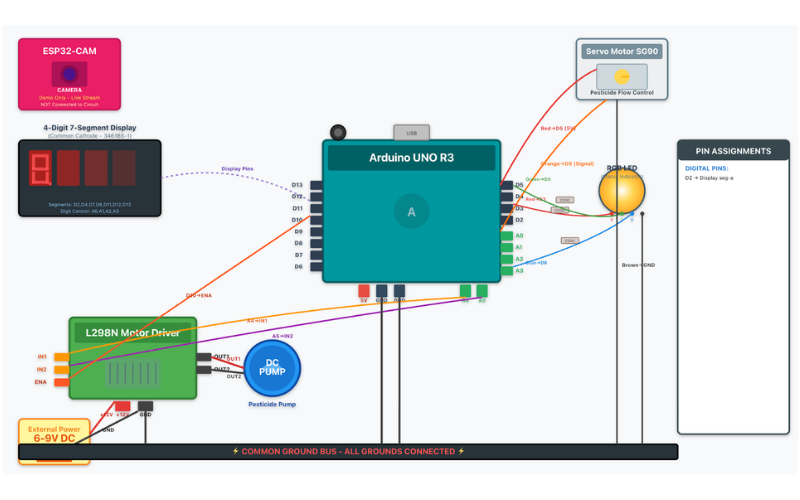
\includegraphics[width=0.7\linewidth]{connection.png}
\caption{Circuit Connection Diagram}
\label{fig:circuit_diagram}
\end{figure}



\section{Error Sources and Mitigation Strategies}

\begin{table}[H]
\centering
\caption{Error Sources and Mitigation Strategies}
\label{tab:errors}
\renewcommand{\arraystretch}{1.3}
\begin{tabularx}{\textwidth}{|X|X|X|}
\hline
\textbf{Error Source} & \textbf{Impact} & \textbf{Mitigation Strategy} \\
\hline
Uneven lighting conditions & Misclassification due to shadows/glare & LED panel lighting; brightness normalisation \\
Model overfitting & Poor generalization to new plant images & Data augmentation; Dropout; fine-tuning \\
Wi-Fi packet loss & Missed spray command & HTTP retry mechanism (3 attempts); local fallback mode \\
Pump pressure variability & Inconsistent spray coverage & Pressure-regulated pump; pre-run calibration \\
Cart positioning error & Nozzle misaligned with plant & Fixed-position markers on garden path \\
Dataset imbalance & Bias toward majority class & Class-weighted loss function; oversampling \\
\hline
\end{tabularx}
\end{table}



% =============================================================
\chapter{HARDWARE AND SOFTWARE REQUIREMENTS}
% =============================================================

\section{Hardware Requirements}

\begin{enumerate}[leftmargin=2em]
    \item \textbf{Processing Unit:} Laptop or PC with minimum Intel i5 (8th Gen) or equivalent, 8 GB RAM, GPU (optional, for faster training — NVIDIA GTX 1650 or higher recommended).
    \item \textbf{Microcontroller:} ESP32 DevKitC v4 (dual-core Xtensa LX6, 240 MHz, 4 MB Flash, 520 KB SRAM).
    \item \textbf{Camera:} Logitech C920 USB Webcam (1080p) or Pi Camera Module v2 (8 MP).
    \item \textbf{Pump:} 12V DC Mini Diaphragm Water Pump (2.4 L/min, max 5 bar).
    \item \textbf{Solenoid Valve:} 12V DC Normally Closed Solenoid Valve (3/8 inch NPT).
    \item \textbf{MOSFET Driver Circuit:} IRF520 N-channel MOSFET with heatsink, 1N4007 flyback diode.
    \item \textbf{Power Supply:} 12V/5A DC adapter (bench testing); 12V LiPo battery pack (field testing).
    \item \textbf{Mobile Cart:} Custom PVC-pipe frame cart with adjustable camera mount.
\end{enumerate}

\section{Software Requirements}

\begin{itemize}[leftmargin=2em]
    \item \textbf{Operating System:} Windows 10/11 or Ubuntu 20.04 LTS.
    \item \textbf{Python:} Version 3.10+ with pip package manager.
    \item \textbf{Libraries:} TensorFlow 2.13, Keras, OpenCV-Python 4.8, NumPy 1.24, Pandas 2.0, Pillow 10.0, Flask 3.0, Matplotlib, Scikit-learn 1.3, SQLite3.
    \item \textbf{IDE:} Visual Studio Code with Python extension; Arduino IDE 2.x.
    \item \textbf{ESP32 Board Package:} esp32 by Espressif (via Arduino Board Manager, version 2.x).
    \item \textbf{ESP32 Libraries:} WiFi.h, WebServer.h, ArduinoJSON 6.x.
    \item \textbf{Dataset:} PlantVillage Tomato Leaf Disease Dataset (Kaggle).
\end{itemize}

% =============================================================
\chapter{EXPECTED RESULTS}
% =============================================================

\section{Expected Model Performance}

Based on the characteristics of the EfficientNetV2-M architecture and the PlantVillage dataset, the following classification performance is anticipated:

\begin{table}[H]
\centering
\caption{Expected Model Performance Metrics}
\label{tab:expected_perf}
\renewcommand{\arraystretch}{1.3}
\begin{tabular}{|l|c|c|c|c|}
\hline
\textbf{Class} & \textbf{Precision} & \textbf{Recall} & \textbf{F1-Score} & \textbf{Support} \\
\hline
Healthy & 0.93 & 0.95 & 0.94 & 360 \\
Moderate Infection & 0.89 & 0.87 & 0.88 & 360 \\
Severe Infection & 0.91 & 0.92 & 0.91 & 360 \\
\hline
\textbf{Overall Accuracy} & \multicolumn{4}{c|}{\textbf{$\geq$ 90\%}} \\
\hline
\end{tabular}
\end{table}

\section{Expected System-Level Performance}

\begin{itemize}[leftmargin=2em]
    \item \textbf{End-to-end latency} (image capture to spray initiation): $\leq 5$ seconds.
    \item \textbf{Pesticide savings}: $\geq 40\%$ reduction in total spray volume compared to uniform spraying on the same set of test plants.
    \item \textbf{Spray accuracy}: Nozzle coverage diameter of 15--20 cm at 30 cm distance, sufficient to cover individual tomato plant canopies.
    \item \textbf{System uptime}: Continuous operation for $\geq 2$ hours per battery charge during field testing.
    \item \textbf{Dashboard data refresh rate}: $\leq 2$ seconds per event.
\end{itemize}

\section{Expected Pesticide Reduction Analysis}

For a test scenario with 10 plants in the following distribution:

\begin{table}[H]
\centering
\caption{Expected Pesticide Reduction: Uniform vs. Intelligent Spraying}
\label{tab:pesticide_reduction}
\renewcommand{\arraystretch}{1.3}
\begin{tabular}{|c|c|c|c|c|}
\hline
\textbf{Plant Distribution} & \textbf{Count} & \textbf{Uniform Spray (s)} & \textbf{Intelligent Spray (s)} & \textbf{Saving} \\
\hline
Healthy & 4 & $4 \times 7 = 28$ & $4 \times 0 = 0$ & 28 s \\
Moderate Infection & 3 & $3 \times 7 = 21$ & $3 \times 3 = 9$ & 12 s \\
Severe Infection & 3 & $3 \times 7 = 21$ & $3 \times 7 = 21$ & 0 s \\
\hline
\textbf{Total} & 10 & \textbf{70 s} & \textbf{30 s} & \textbf{40 s (57\%)} \\
\hline
\end{tabular}
\end{table}

This demonstrates a theoretical pesticide reduction of up to \textbf{57\%} for a typical mixed-health plant population.


\begin{figure}[H]
\centering
    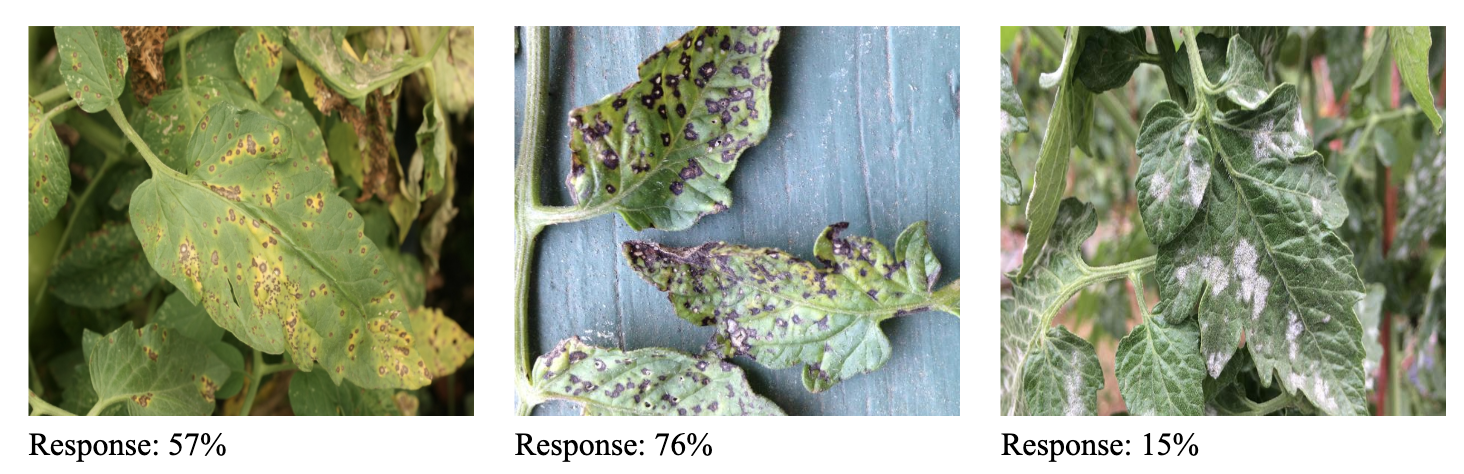
\includegraphics[width=0.87\linewidth]{output.png}
\caption{Sample Output}
\label{fig:sample_output}
\end{figure}

% =============================================================
\chapter{ANALYSIS AND DISCUSSION}
% =============================================================

\section{Expected Performance Trends}

\subsection{Model Training Behaviour}

The following are the trends expected during the two phases of transfer learning:

\begin{itemize}[leftmargin=2em]
    \item \textbf{Phase 1 (base model is frozen)}: Convergence within 5-7 epochs. Expected validation accuracy is 82-85\%
    \item \textbf{Phase 2 (model is fine-tuned)}: Consistent improvement of validation accuracy to $\geq$ 90\%. Significant drop in loss reduction happens after epoch 10 of Phase 2 due to convergence.
    \item \textbf{Risk of over-fitting} is reduced due to use of Dropout layer and data augmentation; training and validation accuracy should not diverge more than 3\%.
\end{itemize}

\subsection{Difficulty Level of Classification Analysis}

The hardest boundary to classify is \textbf{moderate vs severe infection}; there is not much visual distinction between 50\% and 65\% infection of leaf area. It is a difficult problem in case of severity-based leaf classifications and is overcome using fine-augmentation and class-weighting the loss function.

\section{Improvement from Existing Systems}

\begin{enumerate}[leftmargin=2em]
    \item \textbf{Proportionate delivery of pesticides based on severity levels}: The most important novel feature; no such low-cost system is present in reviewed literature.
    \item \textbf{End-to-end deployment of a complete ML-based inference, Wi-Fi communication, hardware actuation and live dashboard in a single prototype}.
    \item \textbf{Cost-efficiency}: Proposed solution is cheaper than $5000~Rs$, while robotic systems in literature have cost orders of magnitude more (\$).
    \item \textbf{Module-based construction of system}: Allows for independent test, upgrades, or replacements of individual modules.
    \item \textbf{Dashboard-based logging and analysis}: Provides actionable insights for farmers/researchers, which is mostly absent in similar systems.
\end{enumerate}

\section{Comparison with Existing Systems}

\begin{table}[H]
\centering
\caption{Comparison of Proposed System with Related Work}
\label{tab:comparison}
\renewcommand{\arraystretch}{1.3}
\begin{tabularx}{\textwidth}{|X|c|c|c|c|c|}
\hline
\textbf{System} & \textbf{Severity-Based Dosing} & \textbf{Real-Time} & \textbf{Low Cost} & \textbf{Dashboard} & \textbf{Crop} \\
\hline
Pansare et al.\ (2025) & \ding{55} & \ding{51} & \ding{55} & \ding{55} & Multiple \\
Ibrahim et al.\ (2025) & \ding{55} & \ding{51} & \ding{55} & \ding{55} & Multiple \\
Ahmed (2024) & \ding{55} & \ding{51} & \ding{51} & \ding{55} & Multiple \\
Kumar et al.\ (2025) & \ding{55} & \ding{55} & \ding{51} & \ding{55} & Tomato \\
\textbf{Proposed System} & \ding{51} & \ding{51} & \ding{51} & \ding{51} & Tomato \\
\hline
\end{tabularx}
\end{table}

\section{Limitations and Mitigations}

\begin{itemize}[leftmargin=2em]
    \item \textbf{Single-crop focus:} The current model is trained only on tomato leaf images. Mitigation: The architecture is designed to be easily re-trained on other crop datasets.
    \item \textbf{Cart navigation is manual:} Full autonomy requires path planning, which is beyond the scope of this project. Future work will integrate an Arduino-based line-following system.
    \item \textbf{Dataset quality dependency:} Model performance degrades in field conditions where lighting is significantly different from training data. Mitigation: Adaptive histogram equalisation during preprocessing.
\end{itemize}

% =============================================================
\chapter{FUTURE SCOPE}
% =============================================================

\section{Potential Enhancements}

\begin{enumerate}[leftmargin=2em]
    \item \textbf{Auto-Navigation Cart:} Adding a line-following or LiDAR sensor to the cart to make it capable of autonomously scanning the plants on a row-by-row basis.

    \item \textbf{Multiclass Crop Disease Classification:} Enhancing the ML model to identify plant diseases from different crops (for example, wheat, rice, chillies).

    \item \textbf{On-Plant Continuous Monitoring:} Installing static cameras in each crop plantation to continuously monitor the plants' health and take preventive measures against disease spread.

    \item \textbf{Edge AI Model Deployment:} Converting the EfficientNetV2-M model to \textbf{TensorFlow Lite} and running it directly on the ESP32-S3 microcontroller equipped with AI capabilities to get rid of Wi-Fi communication.

    \item \textbf{Fertilizer Management:} Developing an advanced algorithm for regulating fertilization dosage using plant growth stage detection as a basis.

    \item \textbf{IoT Platform Integration:} Connecting the web dashboard to cloud IoT platforms such as AWS IoT Core or Google Cloud IoT for predictive analytics.

    \item \textbf{Explainable AI (XAI) Integration:} Integrating Grad-CAM visualization into the project that would provide additional information about leaf sections responsible for the severity level prediction.

    \item \textbf{Renewable Power Source:} Integrating a solar panel for energy harvesting and eliminating the need for a constant connection to a wall charger.
\end{enumerate}
% =============================================================
\chapter{CONCLUSION}
% =============================================================
In this project, we have developed an Intelligent Pesticide Sprinkling System Determined by the Infection Level of Plants—a novel solution based on Computer Vision and Internet of Things to solve the age-old challenge of overuse and waste of pesticides due to blanket application in the current practice of crop protection.

Specifically, this system uses the state-of-the-art \textbf{EfficientNetV2-M} architecture to classify the plant infection levels in real-time into three classes, namely Healthy, Moderate Infection, and Severe Infection, which in turn trigger a proportional pesticide sprinkling process using a 12V DC motor, solenoid valve, and sprayer driven by an \textbf{ESP32} board using the WiFi HTTP Protocol. The system performance is monitored continuously using a web-based GUI dashboard that records all events and maintains cumulative statistics of pesticide consumption.

The important contributions of this project include the following:
\begin{enumerate}[leftmargin=2em]
    \item A \textbf{proportionate closed-loop control mechanism for pesticide sprinkling}, which does not exist in any low-cost precision agriculture solutions.
    \item An \textbf{end-to-end integrated prototype} including the machine learning pipeline, hardware controls, and GUI visualization.
    \item A \textbf{cost-efficient design} (less than Rs. 5,000), affordable to small farmers and educational institutes alike.
    \item An easy-to-scale \textbf{architecture} for extending to more crops and larger scales.
\end{enumerate}


% =============================================================
%  REFERENCES
% =============================================================
\newpage
\begin{thebibliography}{99}

\bibitem{lyseng2023}
R. Lyseng, ``Pesticide waste assigned a number,'' \textit{The Western Producer}, 16 March 2023.

\bibitem{pansare2025}
V. Pansare, A. Kulkarni, and R. Patil, ``Smart agriculture robot for plant disease detection and spraying,'' \textit{International Journal of Scientific Research in Science, Engineering and Technology (IJSRSET)}, vol. 12, no. 3, pp. 45--52, May--June 2025.

\bibitem{healy2025}
M. G. Healy, P. Johnston, and L. O'Connor, ``PestMan: Pesticide management for better water quality,'' \textit{EPA Research Report}, Report No. 480, 2025.

\bibitem{ibrahim2025}
A. S. Ibrahim, M. El-Sayed, and H. Farouk, ``AI--IoT based smart agriculture pivot for plant disease detection and treatment,'' \textit{Scientific Reports}, vol. 15, Article no. 16576, 2025.

\bibitem{kumar2025}
S. Kumar, R. Verma, and P. Singh, ``Deep learning-based ensemble model for accurate tomato leaf disease classification using ResNet50 and MobileNetV2,'' \textit{Scientific Reports}, vol. 15, 2025.

\bibitem{ahmed2024}
S. Ahmed, ``IoT-based intelligent pest management system for precision agriculture,'' \textit{Scientific Reports}, vol. 14, Article no. 31917, 2024.

\bibitem{tan2021}
M. Tan and Q. Le, ``EfficientNetV2: Smaller models and faster training,'' in \textit{Proceedings of the 38th International Conference on Machine Learning (ICML)}, 2021, pp. 10096--10106.

\bibitem{hughes2015}
D. P. Hughes and M. Salathé, ``An open access repository of images on plant health to enable the development of mobile disease diagnostics,'' \textit{arXiv preprint arXiv:1511.08060}, 2015.

\bibitem{mohanty2016}
S. P. Mohanty, D. P. Hughes, and M. Salathé, ``Using deep learning for image-based plant disease detection,'' \textit{Frontiers in Plant Science}, vol. 7, Article 1419, 2016.

\bibitem{ferentinos2018}
K. P. Ferentinos, ``Deep learning models for plant disease detection and diagnosis,'' \textit{Computers and Electronics in Agriculture}, vol. 145, pp. 311--318, 2018.

\bibitem{lecun2015}
Y. LeCun, Y. Bengio, and G. Hinton, ``Deep learning,'' \textit{Nature}, vol. 521, pp. 436--444, 2015.

\bibitem{goodfellow2016}
I. Goodfellow, Y. Bengio, and A. Courville, \textit{Deep Learning}. MIT Press, Cambridge, MA, 2016.

\end{thebibliography}


\end{document}